% Chapter 1

\chapter{Introducción general} % Main chapter title

\label{Chapter1} % For referencing the chapter elsewhere, use \ref{Chapter1} 
\label{IntroGeneral}

%----------------------------------------------------------------------------------------

% Define some commands to keep the formatting separated from the content 
\newcommand{\keyword}[1]{\textbf{#1}}
\newcommand{\tabhead}[1]{\textbf{#1}}
\newcommand{\code}[1]{\texttt{#1}}
\newcommand{\file}[1]{\texttt{\bfseries#1}}
\newcommand{\option}[1]{\texttt{\itshape#1}}
\newcommand{\grados}{$^{\circ}$}

%----------------------------------------------------------------------------------------

%\section{Introducción}
En este capítulo se presenta una breve introducción técnica y se describen la motivación, los objetivos, el alcance y requerimientos del trabajo.
%----------------------------------------------------------------------------------------
\section{Internet de las Cosas}
El término Internet de las Cosas (IoT) describe a una red de interconexión de objetos que incorporan software, hardware y otras tecnologías con el fin de interactuar con otros dispositivos o sistemas a través de Internet. Los objetos físicos que se conectan a esta red, van desde simples sensores de temperaturas domésticos hasta redes de sensores industriales utilizados para el mantenimiento predictivo.

De esta manera, es posible capturar información clave para la detección de patrones de comportamiento que servirán para mejorar la eficiencia de los dispositivos o sistemas a los cuales están conectados. Dada la gran cantidad de sensores y datos recopilados y la alta precisión necesaria para su tratamiento, IoT necesita de tecnologías orientadas al almacenamiento, manipulación y análisis de grandes volúmenes de datos. Una de estas tecnologías que ha penetrado a ritmo acelerado en IoT es la Inteligencia Artificial, ya que al aplicar algoritmos inteligentes, permite inferir conocimiento acerca de los sensores conectados a la red.

Esta información se hace relevante al usuario de alguna forma, ya sea por la realización de alguna acción automática como una notificación o a través de gráficos y valores actuales en los llamados \textit{dashboards} o paneles de control que muestran los datos ya procesados.

Actualmente, IoT está compuesta por una colección dispersa de redes diferentes y con distintos fines \citep{cisco}. Los automóviles, las industrias, los edificios comerciales y residenciales, tienen múltiples redes para vigilar y controlar el funcionamiento de sus sistemas. A medida que IoT evolucione, estas redes se interconectarán con la incorporación de capacidades de seguridad, análisis y administración que se podrán convertir en información y conocimiento. La figura \ref{fig:iotcisco} muestra una proyección de este concepto.

Esto abre una ventana de oportunidades para crear aplicaciones en las áreas de la automatización, el uso de sensores y la comunicación entre máquinas. 
\vspace{1cm}
\begin{figure}[htbp]
	\centering
	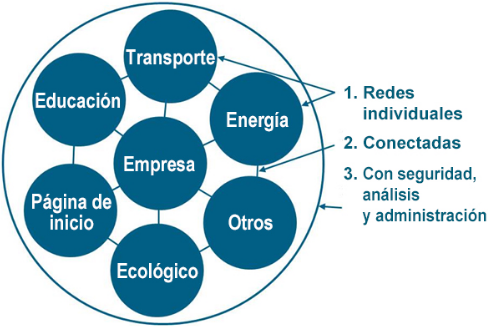
\includegraphics[width=.7\textwidth]{./Figures/iotcisco.png}
	\caption{Futuro de las redes en IoT\protect\footnotemark.}
	\label{fig:iotcisco}
\end{figure}
\vspace{1cm}
\footnotetext{Imagen tomada de: \url{https://www.cisco.com/c/dam/global/es_mx/solutions/executive/assets/pdf/internet-of-things-iot-ibsg.pdf}}

\section{Estado del arte}
Si bien en el mercado existen soluciones para vigilancia de temperaturas aplicadas al área de salud, la mayoría de estos sistemas son de origen importado. Esto hace que los costos y los servicios de mantenimiento sean elevados. Además, en general se comercializan por módulos, por lo que no se proveen soluciones completas.

Ejemplo de algunas empresas que comercializan estos sistemas en nuestro país: 
\begin{itemize}
\item Testo (Alemania) \citep{testo}. 
\item Novus (Brasil) \citep{novus}. 
\item Honeywell (USA) \citep{honeywell}.  
\item Absolut Mobile, empresa nacional que provee soluciones de telemetría a partir de módulos hardware/software importados \citep{absolutmobile}.
\item Bemakoha, empresa nacional que provee productos importados con algunos desarrollos nacionales \citep{bemakoha}.
\end{itemize}

También hay productos de origen nacional, Celsius Patagon \citep{celsius}, empresa rosarina que produce soluciones para IoT, posee un desarrollo para supervisión remota de temperatura. 
 

Casi todas las soluciones necesitan que el cliente tenga un abono mensual para el monitoreo continuo, además de adquirir el hardware correspondiente. Desde este punto de vista, el presente trabajo se destaca especialmente por incorporar una solución integral, de bajo costo, sin gastos de abono y con la característica distintiva que los datos pueden estar guardados en los servidores de la municipalidad de Rosario. Esto lo diferencia de otros sistemas similares en que los datos quedan en poder del fabricante, quien eventualmente, ofrece un portal para poder hacer una visualización. Además, al no ofrecer una solución integral, cada módulo extra incorporado representa un gasto o abono adicional.

En la tabla \ref{tab:comparacionsistemas} se muestra una comparación de algunos ítems importantes entre este trabajo y los sistemas similares de fabricación nacional o importados. En ella se ponen de manifiesto las características de bajo costo y alta prestación del sistema desarrollado.


\begin{table}[h]
	\centering
	\caption[Comparación del trabajo con productos similares importados y nacionales.]{Comparación del trabajo con productos similares importados y nacionales.}
	\begin{tabular}{l l l l}    
	\toprule
	\textbf{Beneficios}    & \textbf{Este trabajo} & \textbf{Importados}& \textbf{Nacionales}\\
	\midrule
Bajo costo del producto & Sí&No &Sí\\
Solución integral& Sí&No &No\\	
No requiere abono mensual & Sí&No &No\\	
No requiere hardware adicional& Sí&No &No\\	
Datos en servidores propios& Sí&No &No\\	
		\bottomrule
		\hline
	\end{tabular}
	\label{tab:comparacionsistemas}
\end{table}

\section{Motivación}
\label{}
El presente proyecto está dirigido a solucionar una problemática existente en la municipalidad de Rosario, donde en el área salud pública funcionan  hospitales, centros de salud, droguerías y bancos de sangre. Todos estos efectores necesitan, para almacenar los insumos médicos, sistemas de refrigeración que provean alta confiabilidad en su prestación.
El buen funcionamiento de estos sistemas es afectado a menudo por cortes de energía, mermas en el rendimiento del equipo compresor, o pérdidas en el sello, ya sea por desgaste de burletes o puertas mal cerradas.
En el área de salud esto resulta crítico puesto que productos medicinales, como hemoproductos o vacunas, pueden perder la eficacia médica. Esto no sólo se traduce en pérdidas económicas, sino también implica que los tratamientos sobre las personas pueden no ser efectivos o que no puedan ser accedidos por la pérdida del material, con el consecuente impacto social que esto representa para el municipio. 
Además, la Administración Nacional de Medicamentos Alimentos y Tecnología Médica (ANMAT), a través de la disposición: ``Buenas Prácticas de Distribución de Medicamentos'', resolución Nº 2069/2018 \citep{anmat}, define un conjunto de prácticas para el transporte y almacenamiento de productos farmacéuticos donde exige trazabilidad, equipamiento para el control y registro continuo de temperaturas con el fin de asegurar las condiciones ambientales de almacenamiento de tales productos. 

La medición a distancia, continua y en tiempo real de estas temperaturas, sumado a un sistema de alerta, aseguran las condiciones legales, minimizan los riesgos y garantizan la disponibilidad de hemoproductos y vacunas seguros en el momento y lugar en que se requieran.

Los equipos y software disponibles en plaza, en su mayoría, son de origen extranjero y su utilización -además de onerosa- implica una dependencia con los fabricantes en términos económicos pero también de criterios. En otras palabras, para trabajar con estos recursos se deben seguir criterios técnico-económicos diseñados para otras latitudes y otras condiciones. Se deben realizar adaptaciones y aproximaciones que implican tareas adicionales y que no siempre son del todo efectivas. El personal destinado a estas tareas debe entrenarse, lo que implica tiempo y esfuerzo. Este entrenamiento debe reforzarse cada vez que el propietario del sistema decide algún cambio o actualización. Por consiguiente, es menester redirigir este esfuerzo a tareas más provechosas.
Se requiere para ello, el desarrollo de tecnología propia destinada a este fin, que pueda ser adaptada a las necesidades de los investigadores locales para evitar la dependencia tecnológica en equipos y en software y reducir en todo lo posible las erogaciones durante la investigación.

\section{Objetivos y alcance}
\label{objetivos}
El propósito de este trabajo es poner en marcha un sistema de registro y visualización de temperaturas para refrigeradores críticos del área salud, con el objetivo de minimizar los riesgos de pérdida de material, mantener la calidad y eficacia médica de los productos y asegurar las condiciones legales exigidas por la autoridad competente.

La solución se compone de las siguientes partes:
\begin{itemize}
\item medición de la temperatura.
\item transporte de los datos.
\item lógica de procesamiento y persistencia de datos.
\item visualización y alarmas.
\end{itemize}


En el trabajo se diseñaron los componentes fundamentales para que el sistema sea capaz de realizar una vigilancia de temperatura de heladeras y freezers pertenecientes a distintos efectores de salud de la ciudad de Rosario. 

Para ello se desarrollaron las siguientes actividades:

\begin{itemize}
\item producción de las placas de circuito impreso para los nodos sensores de temperatura.
\item instalación y configuración de un servidor para proveer la visualización de los datos capturados por los sensores.
\item creación de reglas lógicas para originar las alarmas.
\item instalación de una base de datos en el servidor donde se almacenan las temperaturas y las configuraciones del sistema.
\item configuración de paneles de visualización de temperatura y estado para cada dispositivo conectado al sistema.
\item configuración del envío de las notificaciones de alarmas.
\end{itemize}

Quedan fuera del alcance del trabajo las siguientes características:
\begin{itemize}
\item la provisión de la infraestructura para el transporte de los datos: puntos de acceso a Internet y conexiones a Internet para cada área donde estarán emplazados los sensores.
\item las certificaciones emitidas por las autoridades competentes.
\item el desarrollo de sensores aptos para su instalación en equipos ultrafreezer (-70°C).
\item el almacenamineto de los valores de temperaturas en memorias externas.
\item el uso de baterías para su funcionamiento.
\end{itemize}



\section{Requerimientos}
\label{alcance}


Las actividades mencionadas en la sección \ref{alcance} fueron diagramadas en base a los requerimientos planteados en la planificación. Los mismos se listan a continuación.

\begin{enumerate}
\item Requerimientos de hardware de los nodos
	\begin{enumerate}
	\item Cada nodo estará compuesto por un microcontrolador, un elemento sensor de temperatura y la electrónica asociada para su funcionamiento.
	\item El microcontrolador utilizado deberá estar en fase de producción activa.
	\item El microcontrolador deberá contener capa física WiFi.	
	\item El elemento sensor deberá tener un rango de medición entre -50 y 100 ºC.
	\item El nodo deberá incluir en su circuito un filtro activo de 2º orden para filtrar las componentes de alta frecuencia de la entrada de temperatura.
	\item El nodo deberá incorporar indicadores luminosos de conexión con la red WiFi, conexión con el servidor central e indicador de fuera de rango de temperatura.	
	\end{enumerate}
	
\item Requerimientos del software de los nodos
	\begin{enumerate}
	\item Deberá contener un conjunto de parámetros que identifiquen de forma unívoca al sensor dentro del sistema.	
	\item Los parámetros se deberán almacenar en memoria no volátil.
	\item Deberá gestionar el procesamiento de los valores de temperatura: muestreo cada segundo y promediado cada 600 segundos.	
	\item Deberá incluir parámetros de calibración como offset y ganancia para su futuro contraste con un instrumento patrón.
	\item El nodo deberá incorporar una página web para configuración de parámetros específicos/calibración del sensor.
	\item Deberá incorporar un sistema de actualización remota del firmware.
    \item Deberá ser capaz de conectar distintos modelos de sensores de temperatura.
	\end{enumerate}	
	
\item Requerimientos de seguridad informática
	\begin{enumerate}
	\item La transmisión de los datos se deberá realizar con encriptación, utilizando para ello protocolos de seguridad.
	\item El acceso al sistema de visualización deberá ser con usuario y contraseña.
	\item El acceso a la página web del sensor deberá ser con usuario y contraseña.
	\end{enumerate}	

\item Requerimientos del cliente
	\begin{enumerate}
	\item El sistema de visualización debe incluir roles para distintos usuarios.
		\begin{enumerate}
		\item Rol Administrador: podrá dar alta a usuarios y cambiar sus roles.
	     \item Rol Jefe: podrá cambiar parámetros, visualizar series de tiempo y recibir alertas.
	     \item Rol Operador: sólo podrá visualizar series de tiempo y recibir alertas.
	     \end{enumerate}
	\item El sistema deberá prever la incorporación de otras variables a monitorear, que serán materia de desarrollos futuros de sensores.
	\item El sistema de visualización deberá mostrar claramente la estructura jerárquica geográfica de la empresa.	
	\item El sistema deberá ser escalable para implementar nuevas áreas a monitorear.
		\end{enumerate}
		
\item Requerimientos del sistema de visualización
    \begin{enumerate}
	\item Deberá mostrar la temperatura.
	\item Deberá mostrar el estado del dispositivo que puede ser \textit{online} o fuera de rango.
	\item Deberá mostrar la fecha y hora de la última telemetría enviada al servidor.
	\item Deberá mostrar la configuración de los parámetros de alertas (rangos de temperatura).
	\item Deberá mostrar una vista rápida de los sensores fuera de rango mediante plano en pantalla del área.
	\item Deberá mostrar una tabla con el histórico de alarmas por cada sensor.
    \item Deberá mostrar mediante gráficas la evolución de las temperaturas en el dominio del tiempo con entorno configurable.
    \item Deberá mostrar el lugar de emplazamiento del dispositivo.
	\end{enumerate}	
    

\item Requerimientos de las alarmas
	\begin{enumerate}
	\item Deberá enviar las alarmas discriminadas por efector/área.
	\item Deberá enviar notificaciones ante desplazamientos de la temperatura por encima del rango.
	\item Deberá enviar notificaciones ante desplazamientos de la temperatura por debajo del rango.
	\item Deberá enviar notificaciones ante desconexiones del dispositivo sensor.
	\item Deberá enviar notificaciones ante recupero de la conexión del dispositivo sensor.
	 \end{enumerate}	 

\item Requerimientos de compras
	\begin{enumerate}
	\item Se deberá utilizar la gestión de compras directas para elementos con presupuesto menor a {\$10.000}.
	\item Se deberán realizar las gestiones correspondiente para realizar compras en el exterior.
	\end{enumerate}
\end{enumerate}




%----------------------------------------------------------------------------------------




